\documentclass[12pt]{article}

% More detailed margin control
\usepackage[left=1in,right=1in,top=1in,bottom=1in]{geometry}

% Essential packages
\usepackage{algorithmic}
\usepackage{algorithm}
\usepackage{amsmath}
\usepackage{amssymb} % for triangleq
\usepackage[utf8]{inputenc} % allow utf-8 input
\usepackage[T1]{fontenc}    % use 8-bit T1 fonts
\usepackage{lmodern}
\usepackage{hyperref}       % hyperlinks
\usepackage{url}            % simple URL typesetting
\usepackage{booktabs}       % professional-quality tables
\usepackage{amsfonts}       % blackboard math symbols
\usepackage{nicefrac}       % compact symbols for 1/2, etc.
\usepackage{microtype}      % microtypography
\usepackage{xcolor}         % colors
\usepackage{comment}
\usepackage{enumitem}
\usepackage{subcaption}
\usepackage{graphicx}
\usepackage{amsthm}
\usepackage{lineno}         % for line numbers

\usepackage{nicefrac}       % compact symbols for 1/2, etc.

% Configure line numbers each page
\linenumbers
\modulolinenumbers[5]       % number every 5th line
% \pagewiselinenumbers       % restart line numbers on

% Compatibility for biblatex
\usepackage{csquotes}

% added for Strijov to increase baseline stretch
\usepackage{setspace}
\setstretch{1.35}


% Load biblatex before cleveref
\usepackage{biblatex}
\addbibresource{draft_lib.bib}

\usepackage{cleveref}

% Define custom commands if not already defined
\newcommand{\EE}{\mathbb{E}}
\newcommand{\R}{\mathbb{R}}

% Theorem environments
\newtheorem{assumption}{Assumption}
\newtheorem{lemma}{Lemma}
\newtheorem{proposition}{Proposition}
\newtheorem{theorem}{Theorem}
\newtheorem{corollary}{Corollary}
\newtheorem{definition}{Definition}
\newtheorem{remark}{Remark}

% Comments for co-authors (optional)
\newcommand{\coauthorcomment}[2]{{\color{#1} \textbf{#2}}}

\usepackage{xspace}
\newcommand{\algname}[1]{{\sf  #1}\xspace}
\newcommand{\algnamex}[1]{{\sf #1}\xspace}

% from Mironov
\newcommand{\eqdef}{\stackrel{\Delta}{=}}
\newcommand{\SG}{\mathrm{SG}}
\newcommand{\rd}[3]{\mathrm{D}_{#1}\infdivx*{#2}{#3}}
\newcommand{\rdalpha}[2]{\mathrm{D}_{\alpha}\infdivx*{#1}{#2}}
\newcommand{\renyi}{R\'enyi}
\newcommand{\erfc}{\mathrm{erfc}}
\newcommand{\eps}{\varepsilon}

\usepackage{mathtools}
\DeclarePairedDelimiterX{\infdivx}[2]{(}{)}{#1\;\delimsize\|\;#2}


\usepackage[flushleft]{threeparttable} % http://ctan.org/pkg/threeparttable
\usepackage{colortbl}
\definecolor{bgcolor}{rgb}{0.8,1,1}
\definecolor{bgcolor2}{rgb}{0.8,1,0.8}
\definecolor{niceblue}{rgb}{0.0,0.19,0.56}


% Title and author information
\title{Sign-SGD with Heavy-Tailed Noise and Differential Privacy}

\author{
  Alexey Kravatskiy\\
  \texttt{kravtskii.aiu@phystech.edu}
  \and
  Anton Plusnin\\
  \texttt{plusnin.aa@phystech.edu}
  \and
  Savelii Chezhegov\\
  \texttt{chezhegov.sa@phystech.edu}
  \and
  Alexander Beznosikov\\
  \texttt{beznosikov.an@phystech.edu}
}

\date{\today}

\begin{document}

\maketitle

\begin{abstract}
\iffalse
In the era of large models, federated learning has become indispensable like never before. Sound modern federated learning must meet three key requirements. First and foremost, the whole process of learning must not jeopardize user data, hence be private to given extent. Second, the algorithm must correctly process real-world data, which, in case of Large Language Models (LLMs), means it must tolerate noise with unbounded variance. Third, to ensure applicability, the algorithm must converge under these conditions with high probability, not only in expectation. To address these crucial requirements, we propose a novel modification of Sign version of Stochastic Gradient Descent. In this paper, we demonstrate that it meets all three earlier stated requisites. We start with defining a construction procedure which guarantees differential privacy. Then, we prove algorithm's high-probability convergence on data with heavy-tailed noise. Finally, we show the superior performance of the algorithm in training LLMs in distributed setting.
\fi
Crucial for large-scale models, federated learning faces two major challenges: privacy preservation and high communication costs. While SignSGD addresses the communication issue by transmitting only gradient signs, its only earlier proposed private version lacks proper privacy guarantees and convergence analysis. We construct a new variant of DP-SignSGD that combines Gaussian noise with Bernoulli subsampling to achieve true differential privacy. Our approach satisfies $(\alpha, \varepsilon_R)$-Rényi differential privacy, which can be readily converted to standard $(\varepsilon, \delta)$-privacy guarantees. We demonstrate the algorithm's performance on logistic regression problem and classification of handwritten digits with MLP and CNN. The main challenge remains the tradeoff between precision of a single iteration and the maximum number of privacy-preserving iterations. Our analysis suggests that the sign mechanism's binary output and potential gradient privacy may provide additional privacy guarantees beyond our current calculations. The algorithm can be readily adapted to tighter privacy bounds, and we identify the need for theoretical convergence guarantees as the primary direction for future research.
\end{abstract}

\paragraph{Keywords:} Sign SGD, differential privacy, high-probability convergence, federated learning, heavy-tailed noise.
\paragraph{Idea:} We add Gaussian noise and use privacy amplification by subsampling to make sign-SGD private.

\paragraph{Highlights:}
\begin{enumerate}
\item Sign Stochastic Gradient Descent can be used to train LLMs on real data.
\item Our modification of Sign Stochastic Gradient Descent keeps user data private.
\item Our modification of Sign Stochastic Gradient Descent is applicable to federated setting.
\end{enumerate}

\section{Introduction}
Federated Learning is a useful method to train models that require large amounts of data. Indeed, it is often the case that the data is distributed across multiple devices, like mobile phones \parencite{McMahan2017}, and it is not only costly to collect all the data in one place, but also often unacceptable due to the requirements of privacy. On the other hand, training the model only on the local data for a particular user is impossible, as the model is large and data of one user is insufficient. Hence, a need for a joint training procedure arises. We come to a setting with a server and a number of workers, where each worker has a local dataset. The goal is to train a model on the data from all the workers, without sharing the data between the workers or with the server.

The most obvious way to train a model in a federated setting is to use Stochastic Gradient Descent (\algname{SGD}) \parencite{Robbins1951} by passing the gradient to the server. However, when trasmitting the gradient itself, the communication cost is unaffordably high, and again the data privacy might be violated. To address this issue, one can use the Sign Stochastic Gradient Descent (\algname{SignSGD}) algorithm \parencite{Bernstein2018}. This algorithm transmits only the signs of the coordinates of the gradients, which is much cheaper in terms of communication.

Communication costs aside, clipping the norm of gradient estimate before \algname{SGD} step, which comprises the method called \algname{ClipSGD}, is an another great idea that demonstrates positive empirical results \parencite{Pascanu2013, Goodfellow2016}. Nonetheless, the clipping requires meticulous tuning of the clipping threshold, which was shown to depend on not only iteration number, but also the objective function and the noise \parencite[Theorem $3.1$]{Sadiev2023}. In case of federated learning, the search of the threshold is even more complicated, as the data is distributed across the workers and cannot be used for tuning, and the objective function is more complex due to sophistication and size of the model.

The natural simplification of the clipping is normalization of the gradient, which lies at the core of \algname{NSGD} \parencite{Hazan2015}. \algname{NSGD} outperformed \algname{ClipSGD} on the task of sequence labeling via LSTM Language Models \cite{Merity2017}. Despite this fact, \algname{NSGD}, unlike \algname{ClipSGD}, requires larged batch sizes for convergence, which, however, can be mended by applying momentum \cite{Cutkosky2020}. The major drawback of \algname{NSGD} is the absence of proofs of convergence with high probability. Moreover, the method seems to be far from private.

As to guarantee the privacy is our priority, we opted to base our algorithm on \algname{SignSGD}. The convergence with high probability of \algname{SignSGD} for the heavy-tailed noise has been recently proved \parencite{Kornilov2025}, which makes \algname{SignSGD} a perfect candidate for federated learning. Simultaneously, \algname{SignSGD} has already been used as a base to create an allegedly differentially private algorithm \parencite{Jin2020} (the authors proved differential privacy of only one step of the algorithm). However, in both cases, no proofs for the convergence of the algorithm in the modern federated learning setting were provided.

In this paper, based on the concept of Rényi differential privacy, we develop the idea from \cite{Jin2020} to derive truly differentially-private modification of \algname{SignSGD}, which we naturally call {\scriptsize DP-SIGN}SGD. We show that our algorithm converges with high probability, even in the presence of heavy-tailed noise. Finally, we test the algorithm on the training of MLP and CNN.

\section{Problem statement}
First, we need to state that we work with stochastic optimization.
\paragraph{Stochastic optimization problem.} The stochastic optimization problem for a smooth non-convex function $f:\R^d \to \R$ is:
\begin{eqnarray}
    \min\limits_{x \in \R^d} f(x) := \EE_{\xi \sim \mathcal{S}} [f(x, \xi)],\label{eq: min problem}
\end{eqnarray}
where random variable $\xi$ is sampled from an unknown distribution $\mathcal{S}.$ The gradient oracle returns unbiased gradient estimate $\nabla f (x, \xi) \in \R^d$. In machine learning, for instance, $f(x, \xi)$ is a loss function on a sample $\xi$ \parencite{ShalevShwartz2014}.

The most popular algorithm to solve \eqref{eq: min problem} is Stochastic Gradient Descent (\algname{SGD}) 
 \parencite{Robbins1951}:
\begin{equation}
    x^{k+1} = x^k - \gamma_k \cdot  g^k, \quad g^k := \nabla f (x^k, \xi^k). \notag \label{eq: sgd intro}
\end{equation}
For non-convex functions, the algorithm must stop at the point with sufficiently small gradient norm.
We will apply the algorithm to the federated optimization problem.

\paragraph{Federated optimization problem.}
Let $I = X \times Y$ be a sample space, where $X$ is a space of feature vectors and $Y$ is a label space. For the hypothesis space $\mathcal{W} \subseteq \R^d$, a loss function is defined as $l: \mathcal{W}\times I \rightarrow \R$ which measures the loss of the prediction on the data point $(x,y) \in I$ based on the hypothesis $w \in \mathcal{W}$. For a dataset $D \subset I$, the global loss function $F:\mathcal{W}\to \R$ is defined as
\begin{equation}
F(w) = \frac{1}{|D|}\sum_{(x,y)\in D}l(w;(x,y)).
\end{equation}

In case of distributed optimization, the dataset is split between $M$ workers. Each worker $m$ has a local dataset $D_m \subset I$ and a local function $f_m:\R^d \to \R$ defined as
\begin{equation}
f_m(w)=\frac{1}{|D_m|}\sum_{(x,y)\in D_m}l(w;(x,y)),
\end{equation}
where $|D_m|$ is the size of worker $m$'s local dataset $D_m$.

Thus, our goal is to solve the following federated optimization problem:
\begin{equation}
\min_{w\in \R^d}F(w)~~~~ \text{where}~~~~ F(w) \overset{\mathrm{def}}{=} \frac{1}{M}\sum_{m=1}^{M}f_{m}(w).
\end{equation}

We assume that the data are distributed over the workers uniformly, consequently, $\EE[f_{m}(w)]=F(w)$ for workers' data distribution.

Now, let us introduce the requirements for the algorithm to solve the federated optimization problem.

%\paragraph{Heavy-tailed noise.}
% Noise has bounded $\kappa$-th moment for some $\kappa \in (1,2]$, i.e. $\EE_\xi[\| \nabla f (x, \xi) - \nabla f(x)\|_2^\kappa] \leq \sigma^\kappa$. In % particular, the noise can have unbounded variance when $\kappa < 2$.

\paragraph{Differential privacy}
Additionally, the algorithm must be private. This is guaranteed by $(\epsilon,\delta)$-local differential privacy \cite{Dwork2014}:
\begin{definition}
    Given a set of local datasets $\mathcal{D}$ provided with a notion of neighboring local datasets $\mathcal{N}_{\mathcal{D}}\subset \mathcal{D}\times \mathcal{D}$ that differ in only one data point. For a query function $f: \mathcal{D}\rightarrow \mathcal{X}$, a mechanism $\mathcal{M}:\mathcal{X}\rightarrow \mathcal{O}$ to release the answer of the query is defined to be $(\epsilon,\delta)$-locally differentially private if for any measurable subset $\mathcal{S}\subseteq\mathcal{O}$ and two neighboring local datasets $(D_1,D_2)\in \mathcal{N}_{\mathcal{D}}$,
    \begin{equation}
    \mathbb{P}(\mathcal{M}(f(D_1))\in \mathcal{S}) \leq e^{\epsilon}P(\mathcal{M}(f(D_2))\in \mathcal{S}) + \delta.
    \end{equation}
\end{definition}
    
    A key quantity in characterizing local differential privacy for many mechanisms is the sensitivity of the query $f$ in a given norm $l_{r}$ (we use $l_{2}$), which is defined as
    \begin{equation}\label{sensitivity}
    \Delta_{r} = \max_{(D_1,D_2)\in\mathcal{N}_{\mathcal{D}}}||f(D_1)-f(D_2)||_r.
    \end{equation}

\paragraph{High-probability convergence.}
For given $\delta_{prob} \in (0,1)$, the algorithm must converge with probability at least $1 - \delta_{prob}$.

\section{Theory}
\begin{assumption}[Heavy-tailed noise in gradient estimates]\label{as: pBCM}
    The unbiased estimate $\nabla f (x, \xi)$  has bounded $\kappa$-th moment $\kappa \in (1,2]$ for each coordinate, i.e., $\forall x \in \R^d$: 
    \begin{itemize}
        \item $\EE_\xi [\nabla f (x, \xi)] = \nabla f(x),$
        \item $\EE_\xi [|\nabla f (x, \xi)_i - \nabla f(x)_i|^\kappa] \leq \sigma_i^\kappa, i \in \overline{1,d},$
    \end{itemize}
    where $\Vec{\sigma} = [\sigma_1, \dots, \sigma_d]$ are non-negative constants.
    If $\kappa = 2$, then the noise is called a bounded variance. 
\end{assumption}

\subsection{The Algorithm and the compressor}
The algorithm we are working with can be defined generally as follows:
\begin{algorithm}
    \caption{Stochastic-Sign SGD with majority vote}
    \label{QuantizedSIGNSGD}
    \begin{algorithmic}
        \STATE \textbf{Input}: learning rate $\eta$, current hypothesis vector $w^{(t)}$, $M$ workers each with an independent gradient $\boldsymbol{g}_{m}^{(t)}$, the 1-bit compressor $q(\cdot)$.
        \STATE \textbf{on server:}
        \STATE ~~\textbf{pull} $q(\boldsymbol{g}_{m}^{(t)})$ \textbf{from} worker $m$.
        \STATE ~~\textbf{push} $\tilde{\boldsymbol{g}}^{(t)}= sign\big(\frac{1}{M}\sum_{m=1}^{M}q(\boldsymbol{g}_{m}^{(t)})\big)$ \textbf{to} all the workers.
        \STATE \textbf{on each worker:}
        \STATE ~~\textbf{update} $w^{(t+1)} = w^{(t)} - \eta\tilde{\boldsymbol{g}}^{(t)}$.
    \end{algorithmic}
\end{algorithm}    

Our goal is to find such compressor $q(\cdot)$ that the algorithm is private.

\subsection{Incorrectness of earlier proposed DP-SIGN}
Some time ago, a 1-bit compressor dp-sign \cite{Jin2020} was proposed:

\begin{definition}
    For any given gradient $\boldsymbol{g}_{m}^{(t)}$, the compressor $dp\text{-}sign$ outputs $dp\text{-}sign(\boldsymbol{g}_{m}^{(t)},\epsilon,\delta)$. The $i$-th entry of $dp\text{-}sign(\boldsymbol{g}_{m}^{(t)},\epsilon,\delta)$ is given by
    \begin{equation}\label{dpsignsgd}
    \begin{split}
    &dp\text{-}sign(\boldsymbol{g}_{m}^{(t)},\epsilon,\delta)_{i} =
    \begin{cases}
    1, ~~~~~~~~~ \text{with probability $\Phi\big(\frac{(\boldsymbol{g}_{m}^{(t)})_{i}}{\sigma}\big)$} \\
    -1,  ~~~~~~\text{with probability $1-\Phi\big(\frac{(\boldsymbol{g}_{m}^{(t)})_{i}}{\sigma}\big)$}\\
    \end{cases}
    \end{split}
    \end{equation}
    where $\Phi(\cdot)$ is the cumulative distribution function of the normalized Gaussian distribution; $\sigma = \frac{\Delta_{2}}{\epsilon}\sqrt{2\ln(\frac{1.25}{\delta})}$, where $\epsilon$ and $\delta$ are the differential privacy parameters and $\Delta_2$ is the sensitivity measure.
\end{definition}
As stated in Theorem 5 from \cite{Jin2020}, the $dp\text{-}sign$ mechanism is $(\epsilon, \delta)$-differentially private for any $\epsilon$ and $\delta \in (0, 1)$.

Theorem 6 from \cite{Jin2020} should establish probability of the dissimilarity of majority sign of the gradients and majority sign of the dp-signs:   
\begin{theorem}\label{dp-sign-probabilities}
    Let $u_{1},u_{2},\cdots,u_{M}$ be $M$ known and fixed real numbers. Further define random variables $\hat{u}_{i}=dp\text{-}sign(u_{i},\epsilon,\delta), \forall 1\leq i \leq M$. Then there always exist a constant $\sigma_{0}$ such that when $\sigma \geq \sigma_{0}$, $P(sign(\frac{1}{M}\sum_{m=1}^{M}\hat{u}_{i})\neq sign(\frac{1}{M}\sum_{m=1}^{M}u_{i})) <\big(1-x^2\big)^{\frac{M}{2}}$,
    where $x = \frac{|\sum_{m=1}^{M}u_{m}|}{2\sigma M}$.
\end{theorem}
However, as we recently found out, the theorem is fundamentally flawed, as it makes $\sigma$ a parameter, while it follow from the definition of the $dp\text{-}sign$ compressor that $\sigma$ is a function of $\epsilon$ and $\delta$. 

Let us suppose that there exist $\epsilon$ and $\delta$ such that for $\sigma(\epsilon, \delta)$, the inequality on probability from the theorem holds true. Then, let us walk through the proof to find a precise lower bound for $\sigma$. If this bound is lower than $\sigma(\epsilon, \delta)$, the theorem is indeed correct.

In the proof of Theorem 6, the authors needed to find the lower bound for the following expression:
$$\frac{1}{\sqrt{2\pi}\sigma}\bigg[\bigg|\sum_{m=1}^{M}u_{m}\bigg|e^{-\frac{u_{1}^2}{2\sigma^2}}+\bigg|\sum_{m=2}^{M}u_{m}\bigg|\bigg[e^{-\frac{(\sum_{m=2}^{M}u_{m})^2}{2\sigma^2}}-1\bigg]\bigg]$$

Instead of taking limit $\sigma \to \infty$ as they did, we will use the well known relation $e^{-x^2} \geq 1 - x^2$. After applying it to the earlier mentioned expression and making some trivial transformations, we get the following:
$$\sigma^2 \geq
\frac{7}{5} \left(u_1^2 + \left|\sum_{m=1}^M u_m\right|^2 + \frac{|u_1|^3}{\left|\sum_{m=1}^M u_m\right|}\right).
$$

It is a sufficient condition, not a necessary one. However, it reflects the key features of the condition on $\sigma$. $\frac{|u_1|^3}{\left|\sum_{m=1}^M u_m\right|}$ is an extremely unreliable term, as $|u_1|$ may be high, especially for heavy-tailed noise, while $\left|\sum_{m=1}^M u_m\right|$ may be small (it is easy to construct an appropriate example for the case of 3 workers). Hence, the bound on $\sigma$ is not only high, but also unstable. Consequently, we have no proofs whatsoever of the convergence of the algorithm.

Moreover, our misgivings are supported by the fact that in an updated version \cite{Jin2024} of the article \cite{Jin2020}, the authors have removed all mentions of dp-sign.

The problems with convergence of dp-sign are not limited by the incorrect Theorem 6. The authors have overlooked another issue of utmost importance. Proving the $(\epsilon, \delta)$ differential privacy of dp-sign, they did so for only one call of dp-sign operator. However, according to \cite{Dwork2014} (Theorem 3.16), the overall privacy of running dp-sign $T$ times is $(T \epsilon, T \delta)$. Consequently, when we set target $\epsilon \approx 10$, $\delta \approx 10^-5$, as is recommended for machine learning purposes \cite{Ponomareva2023}, for $T = 100$ we get 100 times lower $\epsilon$ and $\delta$ for dp-sign. Judging by our experiments, this destroys convergence. That is intuitive: high noise for low $(\epsilon, \delta)$ leads to poorer convergence, and this forces us to use still lower $(\epsilon, \delta)$ to preserve the required level of privacy during the run of the algorithm.

To the best of our knowledge, there are no differentially private versions of sign-sgd reported except this incorrect dp-sign. As Gaussian noise is still the best mechanism to ensure differential privacy (Laplace noise and exponential mechanism complicate convergence), we preserve the idea of dp-sign. However, we drastically change the privacy analysis to make $\sigma$ small enough for the algorithm to converge.

\subsection{Rényi Differential privacy}
To make an economical use of differential privacy, we have to introduce another type of differential privacy, which gives more tight bounds on composition.
    \begin{definition}[\renyi\ divergence \cite{Mironov2017}] Let $P$ and $Q$ be two distributions on $\mathcal{X}$ defined over the same probability space, and let $p$ and $q$ be their respective densities. The \renyi\ divergence of a finite order $\alpha\neq 1$ between $P$ and $Q$ is defined as
    \[
    \rdalpha{P}{Q}\eqdef \frac1{\alpha-1}\ln \int_{\mathcal{X}} q(x)\left(\frac{p(x)}{q(x)}\right)^{\alpha}\,\mathrm{d}x.
    \]
    \renyi\ divergence at orders $\alpha=1,\infty$ are defined by continuity.
    \end{definition}
    
    
    \begin{definition}[\renyi\ differential privacy (RDP) \cite{Mironov2017}] We say that a randomized mechanism $\mathcal{M}\colon \mathcal{S}\to\mathcal{R}$ satisfies $(\alpha,\eps)$-\renyi\ differential privacy (RDP) if for any two \emph{adjacent} inputs $S,S'\in \mathcal{S}$ it holds that
    \[
    \rdalpha{\mathcal{M}(S)}{\mathcal{M}(S')}\leq \eps.
    \]
    \end{definition}

    The notion of adjacency between input datasets is domain-specific and is usually taken to mean that the inputs differ in contributions of a single individual. In this work, we will use this definition and call two datasets $S, S'$ to be adjacent if $S' = S \cup \{x\}$ for some $x$ (or vice versa).
    
    \begin{definition}[Sampled Gaussian Mechanism (SGM) \cite{mironov2019SGM}] Let $f$ be a function mapping subsets of $\mathcal{S}$ to $\mathbb{R}^d$. We define the Sampled Gaussian mechanism (SGM) parameterized with the sampling rate $0<q\leq 1$ and the noise $\sigma>0$ as
        \[
        \SG_{q,\sigma}(S)\eqdef f(\{x\colon x\in S \textrm{ is sampled with probability } q\})+\mathcal{N}(0,\sigma^2\mathbb{I}^d),
        \]
    where each element of $S$ is sampled independently at random with probability $q$ without replacement, and $\mathcal{N}(0,\sigma^2\mathbb{I}^d)$ is spherical $d$-dimensional Gaussian noise with per-coordinate variance $\sigma^2$.
    \end{definition}
    
From Section 3.3 (\textit{``Numerically stable computations``}) of \cite{mironov2019SGM}, for each integer $\alpha \geq 1$, SGM applied to a function with $\Delta_2\leq1$ is $(\alpha, \eps_R)$-RDP for the following $\eps_R$:
\begin{equation}\label{eq:renyi_eps_guarantee}
\eps_R = \frac{1}{\alpha - 1} \log\left(\sum_{k=0}^{\alpha} {\alpha \choose k}  (1-q)^{\alpha-k}q^{k} \exp\left(\frac{k^2 - k}{2\sigma^2}\right)\right)
\end{equation}

Clearly, if $\Delta_2 > 1$ for a mechanism, $\sigma := \Delta_2 \sigma$ will deliver the same $(\alpha, \eps_R)$-RDP.

If an $(\alpha, \eps_R)$-RPD mechanism is applied $T$ times, by adaptive sequential composition \cite{Mironov2017}, we get $(\alpha, T\eps_R)$-RDP of the procedure. From \textit{Proposition 3} from \cite{Mironov2017}, it follows that the procedure is also $(\eps_R + \frac{\log1/\delta}{\alpha - 1}, \delta)$-differentially private for any $0 \leq \delta \leq 1$. Thus, the procedure is $(\eps, \delta)$-differntial privacy, if $(\alpha, \eps_R)$ satisfy:

\begin{equation}\label{eq:renyi_eps_requirement}
\eps_R \leq \eps/T - \frac{\log 1/\delta}{T(\alpha - 1)}
\end{equation}

As convergence of the algorithm depends only on $\sigma$, while $\alpha$ is an internal parameter, we are interested in finding the minimal $\sigma$. This we achieve via grid search on integer $1\leq \alpha \leq 20$ and $0.5 \leq \sigma \leq 3$. An example can be seen in Figure~\ref{fig:grid_sigma}.
\begin{figure}[h]
    \centering
    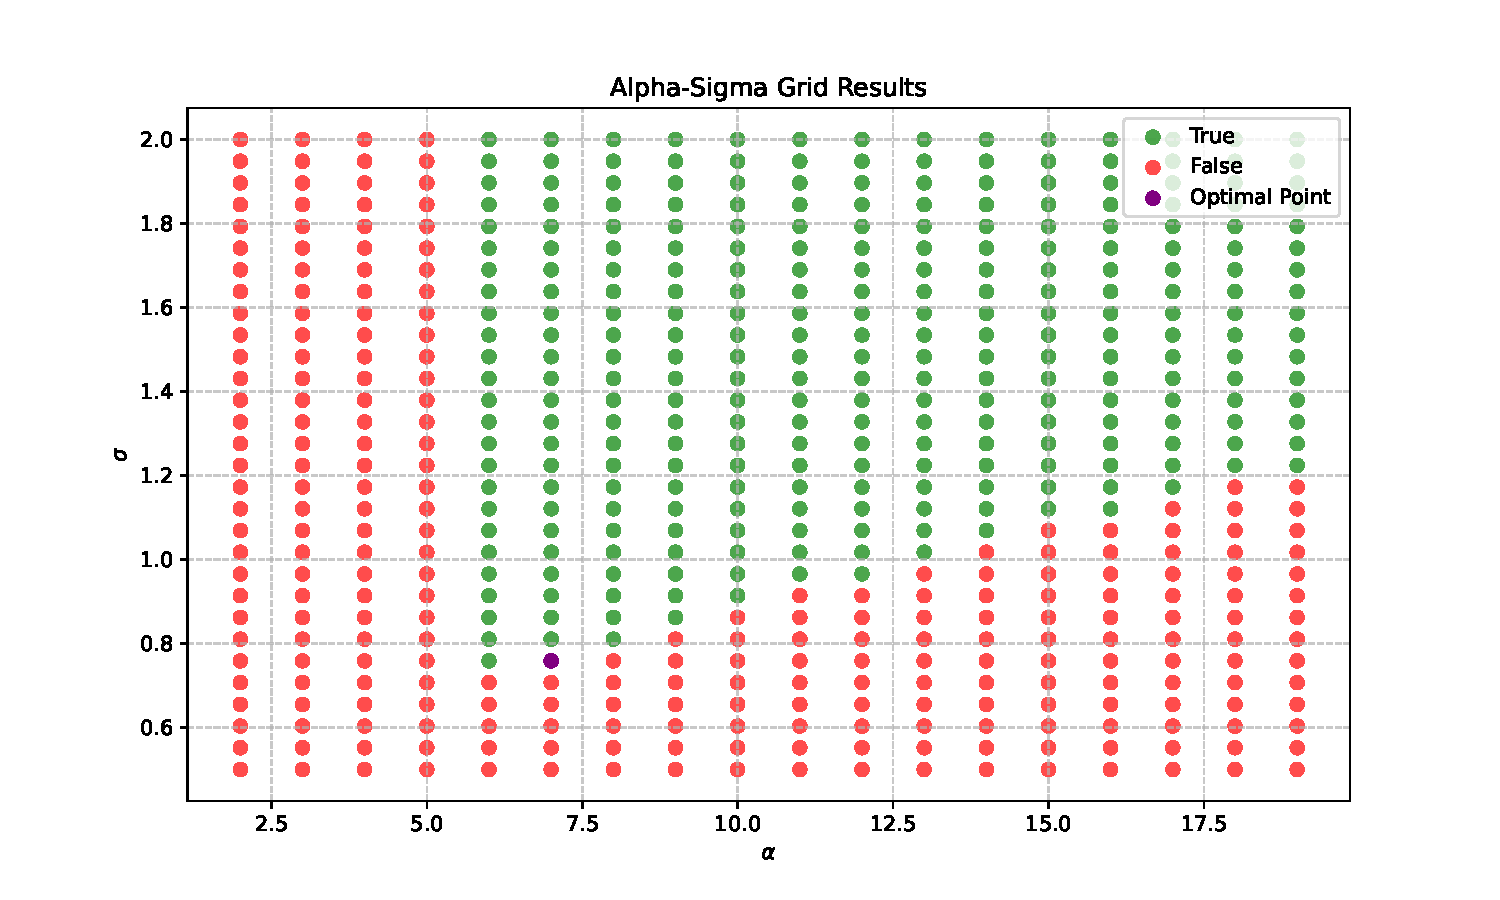
\includegraphics[width=0.98\textwidth]{../figs/valid_sigma.pdf}
    \caption{Finding the minimal $\sigma$ for SGM with $\Delta_2 \leq 1$, sampling rate $q = 1/300$, and $T = 1000$}
    \label{fig:grid_sigma}
\end{figure}

Judging by the chart, there is no need in searching among $\alpha \in \R$: \textit{Case II. Fractional $\alpha$} from \cite{mironov2019SGM} gives a series expression to obtain a bound for $\eps_R$, and the series is continuous on $\alpha$. Continuous borderline on \ref{fig:grid_sigma} implies that $\sigma$ we get by the grid search is close to the optimum.

\subsection{Constructing DP-SIGN}
Let us define {\scriptsize DP-SIGN} \ref{dp-sign-precise}. From the previous section, $(\eps, \delta)$-privacy of {\scriptsize DP-SIGN} immediately follows.
\newcommand{\gradg}{\boldsymbol{g}}
\begin{algorithm}
    \caption{DP-SIGN compressor}
    \label{dp-sign-precise}
    \begin{algorithmic}
        \STATE \textbf{Input}: coordinate $w$, loss function $l$, user database $D$, $(\eps, \delta)$-privacy requirement, number of iterations $T$, sampling rate $q$, clipping level $C$.
        \STATE Prepare subsample $S$: add each element $(x, y) \in D$ with probability $q$.
        \STATE Compute the gradient $\gradg$ of the subsample: $\frac{1}{|S|}\sum_{(x,y)\in S}l(w;(x,y))$. If $S$ is empty, let $\gradg = 0$.
        \STATE If $||\gradg||_2 > C$: $\gradg = C\frac{\gradg}{||\gradg||_2}$.
        \STATE Grid search $\sigma(q, T, \eps, \delta)$ to satisfy \eqref{eq:renyi_eps_guarantee} and \eqref{eq:renyi_eps_requirement}.
        \STATE $\gradg_{priv}$ = $\gradg + \mathcal{N}(0,(C\sigma)^2\mathbb{I}^d)$
        \STATE \textbf{Output}: $sign(\gradg_{priv})$
    \end{algorithmic}
\end{algorithm}

\begin{theorem}\label{prop:dp_guarantee}
Let $l(\cdot;\cdot)$ be a loss function and let $\eps > 0$, $\delta \in (0,1)$. Then applying $T$ times dp-sign($w_i$, $l$, $D$, $(\eps, \delta)$, $T$, $q$, $C$) in different points $w_i$ on a user database $D$ with a fixed sampling rate $q$ and fixed clipping level $C > 0$ is $(\eps, \delta)$-differentially private.
\end{theorem}
\begin{proof}
$\gradg_{priv}$ is private due to the satisfaction of \eqref{eq:renyi_eps_guarantee} and \eqref{eq:renyi_eps_requirement}. As RDP preserves under post-processing (\cite{Mironov2017}), $sign(\gradg_{priv})$ is also $(\alpha, \eps_R)$-RPD, which entails $(\eps, \delta)$-dp for all $T$ iterations.
\end{proof}


\section{Experiments}
In this section, we present the experimental results for the methods we discussed in Sections 2 and 3. First, we appy the algorithms to a classic machine learning problem. Then, we test the algorithms on the training of Large Language Models.

\subsection{Synthetic noise.}
We test our algorithm on the method of logistic regression for UCI Mushroom Dataset. The dataset consists of 6,449 training samples and 1,625 testing samples. Each sample has $d = 112$ features, and represents a mushroom either poisonous or edible. We apply different algorithms to train the logistic regression model. The algorithms are run for $T = 100000$ iterations on 10 workers, with training data distributed between the workers equally. We compare the cases when there is no noise, when the noise is normal with $\sigma = 1/4$, and when the noise is coordinatewise Lévy stable with $\sigma_l = 1/4$, $\alpha_l=1.6$, which corresponds to $\kappa=1.5$, and $\beta_l=0$ (this distribution is defined by its characteristic function $\varphi(t)=\exp\left(-0.25^{1.6}|t|^{1.6})\right)$. For private algorithms, we set $\epsilon \approx 10$, $\delta \approx 1/n^{1.1}$, where $n$ is the size of local user database, as is recommended for machine learning purposes \cite{Ponomareva2023}. We set the learning rate $\gamma = 1/\sqrt{d T}$ for SGD, sign-SGD, and {\scriptsize DP-SIGN}SGD. The results are presented in \ref{fig:logreg}.
\begin{figure}[h]
    \centering
    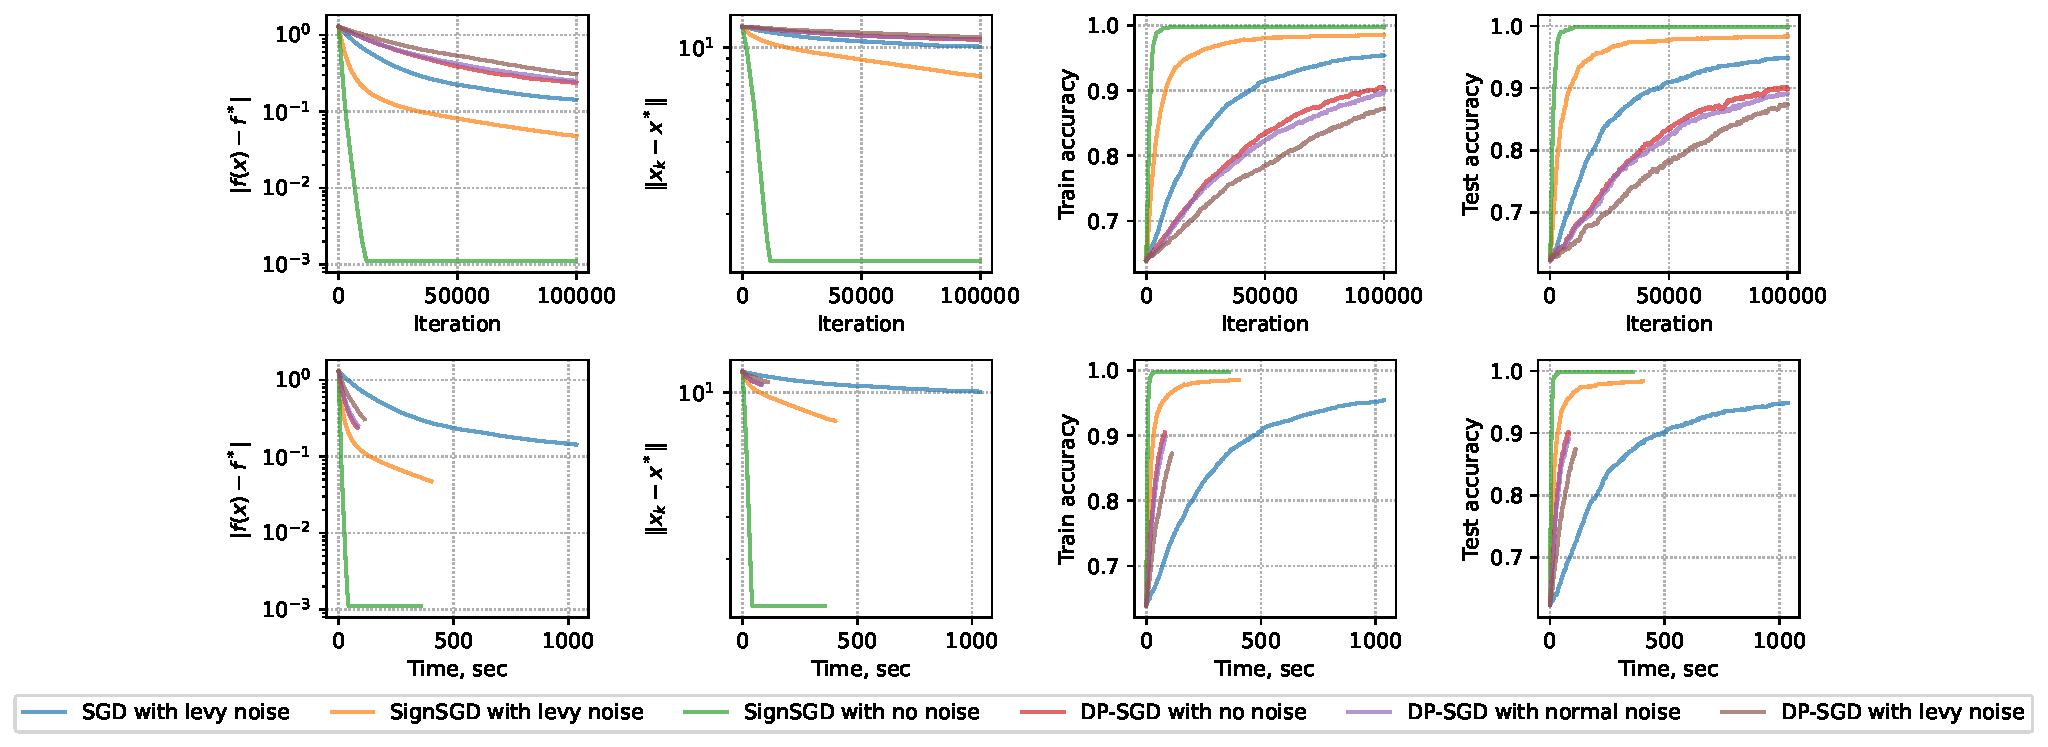
\includegraphics[width=1\textwidth]{../figs/v17_10_workers_long.pdf}
    \caption{Logistic regression on UCI Mushroom Dataset.\newline Performance of SGD, SignSGD, and {\scriptsize DP-SIGN}SGD with majority voting.}
    \label{fig:logreg}
\end{figure}

As we see, {\scriptsize DP-SIGN}SGD does converge, even under heavy-tailed noise.

\subsection{DP-Sign: Comparison}
Having verified Sign-SGD, we test dp-sign on the same dataset. We present three variants of the dp-sign:
\begin{enumerate}
    \item DP-SignSGD from \cite{Jin2020} with unrectified $(\epsilon, \delta)$. The algorithm converges, but is not sufficiently private, as we highlighted earlier.
    \item DP-SignSGD from \cite{Jin2020} with rectified $(\epsilon / T, \delta /T)$, where $T$ is 1000. The algorithm is now private, but does not converge.
    \item Our modification of DP-SignSGD. We used Rényi differential privacy \cite{Dwork2014}. This type of privacy can be easily converted to classical differential privacy, but has a more temperate deterioration of privacy during the sequential composition: the noise $\sigma \sim \sqrt{T}$ instead of $\sigma \sim T$. We will expand Theory and introduce there this algorithm, when it will be ready. For now, it as dp-sign does not converge.
\end{enumerate}
\begin{figure}[h]
    \centering
    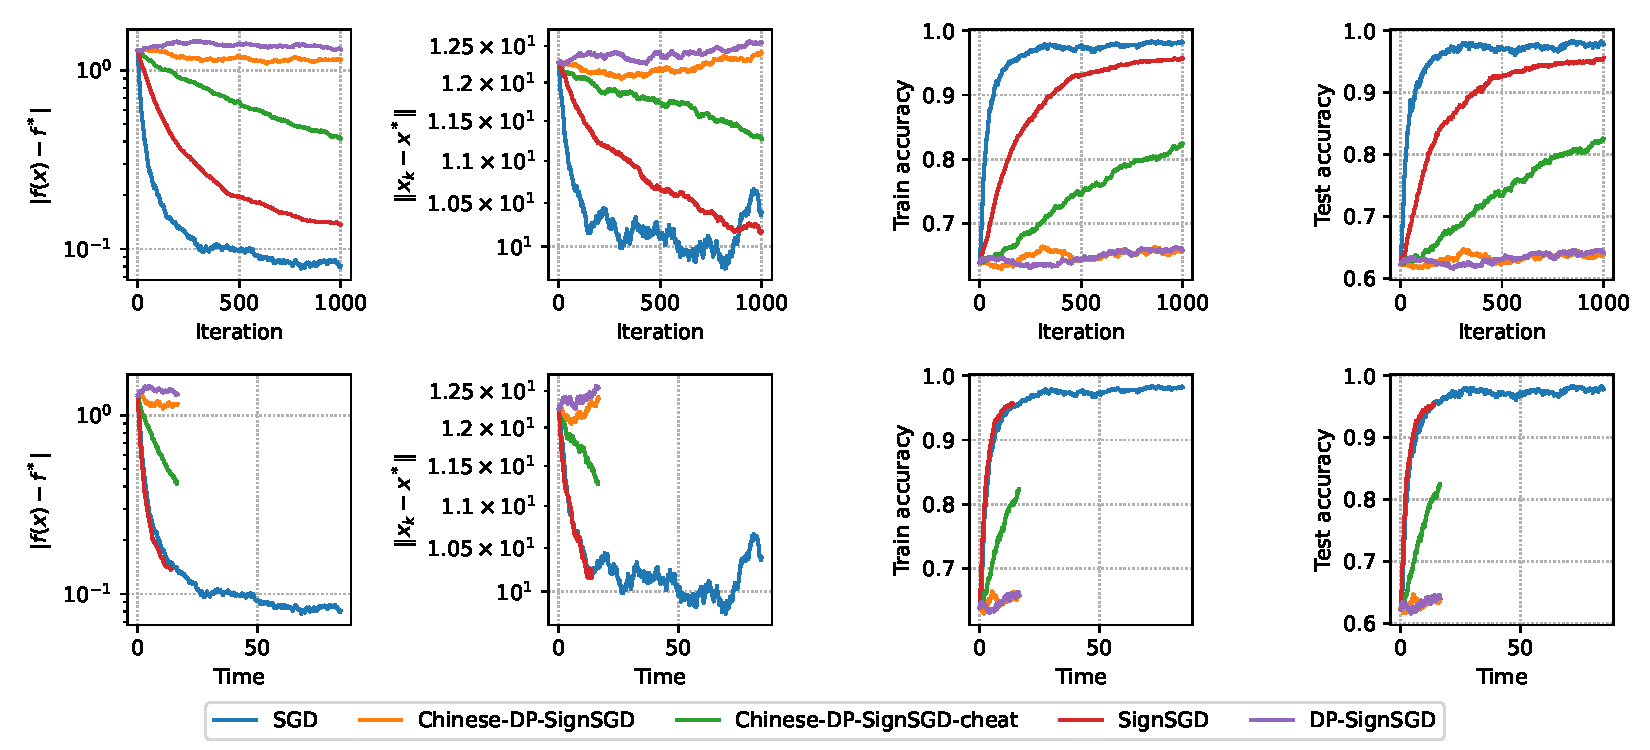
\includegraphics[width=0.98\textwidth]{../figs/dps_diverge.pdf}
    \caption{Logistic regression on UCI Mushroom Dataset.\newline Performance of SGD, SignSGD and different variants of DP-SignSGD with majority voting.}
    \label{fig:dp-diverges}
\end{figure}

\begin{table}\label{compare-chinese}
    \centering
        \small
% 		\scriptsize
    \caption{\small DP-Sign SGD methods}

\label{tab:dpsign_methods}    
		\begin{threeparttable}
			\begin{tabular}{|c|c c c|}
			\hline
				Method & Citation & Is $(\epsilon, \delta)$ private & Converges \\
                \hline
                \hline
				\algname{ChineseDP-SignSGD-cheat} & \parencite{Jin2020} & No & Yes\\
                \hline
                \algname{ChineseDP-SignSGD rectified} & \parencite{Jin2020} & Yes & No\\
                \hline
				\rowcolor{bgcolor2}\algname{Rényi DP-SignSGD} & \textbf{This paper} & Yes & Yes\\
			    \hline
			\end{tabular}
		\end{threeparttable}
\vspace{-2mm}
\end{table}

Thus, we have the following table \ref{tab:dpsign_methods}.

\section{Conclusion}
We have highlighted the deficiencies of the previous approach of working with dp-sign-SGD. With a use of Rényi differential privacy and advanced numerically-produced bounds for Sampled Gaussian Mechanism, we have consturcted a privacy accountant that makes dp-sign-SGD converge and private, which, to the best of our knowledge, has never been done before. 

\section{Acknowledgments}
We will fill this section when we are done with the article.

\appendix
\section{Additional Proofs}
We will present them after we complete the tests and finalize the algorithm.

\printbibliography

\end{document}